
%\documentclass[3p,twocolumn]{elsarticle}
\documentclass[12pt]{iopart}

\usepackage{xspace}
\usepackage{vistrails}
%\usepackage{amsmath}
%\usepackage{amssymb}
%\usepackage{amsmath}
\usepackage{color}
\usepackage{hyperref}
%\bibliographystyle{unsrt} %bibtex style according to iop latex guidelines
%\usepackage{harvard}
%\bibliographystyle{jphysicsB} %bibtex style according to iop latex guidelines

\renewcommand{\vistrailspath}{http://alps.comp-phys.org/vistrails/run_vistrails.php}
\renewcommand{\vistrailsdownload}{http://alps.comp-phys.org/vistrails/download.php}

\newcommand{\eg}{e.g.,\xspace}
\newcommand{\ie}{i.e.,\xspace}
\newcommand{\etc}{etc.\@\xspace}
% \newcommand{\etal}{~et~al.\@\xspace}

\newcommand{\markref}[1]{#1}
\newcommand{\freiremarkref}[1]{#1}
\newcommand{\me}{Juliana Freire}
\newcommand{\meabbrev}{J.~Freire}


\begin{document}

\title{The ALPS project release 2.0: \\ open source software for strongly correlated systems}


\newcounter{affiliation}
% with email addresses
%\newcommand{\myauthor}[3]{#2 {\small (#3)}$^{#1}$}
% without them
\newcommand{\myauthor}[3]{#2$^{#1}$}
\newcommand{\myaddress}[2]{\address{\refstepcounter{affiliation} $^{\arabic{affiliation}}$#2 \label{#1}}}

\author{
	\myauthor{\ref{eth}}{B. Bauer}{bauerb@phys.ethz.ch}
	\myauthor{\ref{colorado}}{L.~D.~Carr}{lcarr@mines.edu}
	\myauthor{\ref{graz}}{H.G. Evertz}{evertz@tugraz.at}
	\myauthor{\ref{wyoming}}{A. Feiguin}{afeiguin@uwyo.edu}
	\myauthor{\ref{utah}}{J. Freire}{juliana@cs.utah.edu}
	\myauthor{\ref{goettingen}}{S.~Fuchs}{fuchs@theorie.physik.uni-goettingen.de}
	\myauthor{\ref{eth}}{L. Gamper}{gamperl@gmail.com}
	\myauthor{\ref{eth}}{J. Gukelberger}{gukelberger@phys.ethz.ch}
	\myauthor{\ref{columbia}}{E. Gull}{gull@phys.columbia.edu}
	\myauthor{\ref{bonn}}{S.~Guertler}{guertler@th.physik.uni-bonn.de}
	\myauthor{\ref{eth}}{A.~Hehn}{hehn@phys.ethz.ch}
	\myauthor{\ref{jaea},\ref{crest}}{R.~Igarashi}{rigarash@hosi.phys.s.u-tokyo.ac.jp}
	\myauthor{\ref{eth}}{S.V.~Isakov}{isakov@phys.ethz.ch}
	\myauthor{\ref{utah}}{D. Koop}{dakoop@cs.utah.edu}
	\myauthor{\ref{eth}}{P.N. Ma}{pingnang@phys.ethz.ch}
	\myauthor{\ref{eth},\ref{utah}}{P.~Mates}{mates@sci.utah.edu}
	\myauthor{\ref{tokyo}}{H. Matsuo}{halm@looper.t.u-tokyo.ac.jp}
	\myauthor{\ref{paris}}{O. Parcollet}{parcolle@spht.saclay.cea.fr}
	\myauthor{\ref{affpol}}{G.~Pawlowski}{gpawlo@amu.edu.pl}
	\myauthor{\ref{epfl}}{J.D.~Picon}{jean-david.picon@epfl.chl}
	\myauthor{\ref{harvard},\ref{eth}}{L.~Pollet}{pollet@phys.ethz.ch}
	\myauthor{\ref{goettingen}}{T.~Pruschke}{pruschke@theorie.physik.uni-goettingen.de}
	\myauthor{\ref{utah}}{E.~Santos}{emanuele@sci.utah.edu}
	\myauthor{\ref{virginia}}{V.W.~Scarola}{scarola@vt.edu}
	\myauthor{\ref{lmu}}{U.~Schollw\"ock}{schollwoeck@lmu.de}
	\myauthor{\ref{utah}}{C.~Silva}{csilva@sci.utah.edu}
	\myauthor{\ref{eth}}{B.~Surer}{surerb@phys.ethz.ch}
	\myauthor{\ref{tokyo},\ref{crest}}{S. Todo}{wistaria@ap.t.u-tokyo.ac.jp}
	\myauthor{\ref{stationq}}{S.~Trebst}{trebst@kitp.ucsb.edu}
	\myauthor{\ref{eth}}{M.~Troyer}{troyer@ethz.ch}\footnote{Corresponding author: troyer@comp-phys.org}
	\myauthor{\ref{colorado}}{M.~L.~Wall}{mwall@mymail.mines.edu}
	\myauthor{\ref{eth}}{P. Werner}{werner@phys.ethz.ch}
	\myauthor{\ref{rwth},\ref{stuttgart}}{S. Wessel}{wessel@phys.ethz.ch}
}

\myaddress{eth}{Theoretische Physik, ETH Zurich, 8093 Zurich, Switzerland}
\myaddress{colorado}{Department of Physics, Colorado School of Mines, Golden, CO 80401, USA}
\myaddress{graz}{Institut f\"ur Theoretische Physik, Technische Universit\"at Graz, A-8010 Graz, Austria}
\myaddress{wyoming}{Department of Physics and Astronomy, University of Wyoming, Laramie, Wyoming 82071, USA}
\myaddress{utah}{Scientific Computing and Imaging Institute, University of Utah, Salt Lake City, Utah 84112, USA}
\myaddress{goettingen}{Institut f\"ur Theoretische Physik, Georg-August-Universit\"{a}t G\"{o}ttingen, G\"{o}ttingen, Germany}
\myaddress{columbia}{Columbia University, New York, NY 10027, USA}
\myaddress{bonn}{Bethe Center for Theoretical Phyics, Universit\"{a}t Bonn, Bonn, Germany}
\myaddress{jaea}{Center for Computational Science \& e-Systems, Japan Atomic Energy Agency, 110-0015 Tokyo, Japan}
\myaddress{crest}{Core Research for Evolutional Science and Technology, Japan Science and Technology Agency, 332-0012 Kawaguchi, Japan}
\myaddress{harvard}{Physics Department, Harvard University, Cambridge 02138, Massachusetts, USA} 
\myaddress{paris}{Institut de Physique Theorique, CEA/DSM/IPhT-CNRS/URA 2306, CEA-Saclay, F-91191 Gif-sur-Yvette, France} 
\myaddress{affpol}{Faculty of Physics, A. Mickiewicz University, ul. Umultowska 85, 61-614 Poznan, Poland}
\myaddress{epfl}{Institute of Theoretical Physics, EPF Lausanne, CH-1015 Lausanne, Switzerland}
\myaddress{virginia}{Department of Physics, Virginia Tech, Blacksburg, Virginia 24061, USA}
\myaddress{lmu}{Department for Physics, Arnold Sommerfeld Center for Theoretical Physics and Center for NanoScience, University of Munich,  80333 Munich, Germany}
\myaddress{tokyo}{Department of Applied Physics, University of Tokyo, 113-8656 Tokyo, Japan}
\myaddress{stationq}{Microsoft Research, Station Q, University of California, Santa Barbara, CA 93106, USA}
\myaddress{rwth}{Institute for Solid State Theory, RWTH Aachen University, 52056 Aachen, Germany}
\myaddress{stuttgart}{Institut f\"ur Theoretische Physik III, Universit\"at Stuttgart, Pfaffenwaldring 57, 70550 Stuttgart, Germany}

\begin{abstract}
We present release 2.0 of the ALPS (Algorithms and Libraries for Physics Simulations)
project, an open source software project to develop
libraries and application programs for the simulation of strongly
correlated quantum lattice models such as quantum magnets, lattice
bosons, and strongly correlated fermion systems. Development is
centered on common XML and HDF5 data formats, libraries to
simplify and speed up code development, common evaluation and plotting tools, and
simulation programs. The programs enable non-experts to start carrying
out serial or parallel numerical simulations by providing basic implementations of the
important algorithms for quantum lattice models: classical and quantum
Monte Carlo (QMC) using non-local updates, extended ensemble
simulations, exact and full diagonalization (ED), the
density matrix renormalization group (DMRG) both in a static version and a dynamic time-evolving block decimation (TEBD) code, and quantum Monte Carlo solvers for dynamical mean field theory (DMFT). Major changes in release 2.0 include the use of HDF5 for binary data, evaluation tools in Python, support for the Windows operating system, the use of CMake as build system and binary installation packages for Mac OS X and Windows, and integration with the VisTrails workflow provenance tool.
The software is available from our web server at \url{http://alps.comp-phys.org/}.
\end{abstract}

\section{Introduction}
\label{}

In this paper we present release 2.0 of the ALPS project  (Algorithms and Libraries for Physics Simulations), an open source software development project for strongly correlated lattice models. We will present a short overview  and focus on new features compared to the previous releases \cite{ALPS1.2,ALPS1.3}.

Quantum fluctuations and competing interactions in quantum many body
systems lead to unusual and exciting properties of strongly correlated
materials such as quantum magnetism, high temperature
superconductivity, heavy fermion
behavior, and topological quantum order.
The strong interactions make accurate analytical treatments hard and 
direct numerical simulations are essential to increase our understanding of the unusual
properties of these systems. 

The last two decades have seen tremendous progress in the development of
algorithms.  Speedups of many orders of magnitude have been 
achieved \cite{Evertz03,Troyer03,White1992,Schollwock2005,vidal1,vidal2,Daley2004,White2004,Rubtsov04,Rubtsov05,Werner06,Werner06Kondo, Gull08_ctaux}. These
advances often come at the cost of increased algorithmic
complexity and challenge the current model of program development in
this research field. In contrast to other research areas, in which
large ``community codes'' are being used, the field of strongly
correlated systems has so far been based mostly on single codes developed by
individual researchers for particular projects. While simple
algorithms used a decade ago could be easily programmed by a beginning
graduate student in a matter of weeks, it now takes substantially
longer to master and implement the new algorithms.  At the same time, the use of numerical approaches is increasing.  

The ALPS project aims to
overcome the problems posed by the growing complexity of algorithms
and the specialization of researchers to single algorithms through
an open-source software development initiative. Its goals are to simplify the development of new codes through libraries and evaluation tools, and to help users with ``black box'' codes of some of the most popular algorithms. To achieve these goals the ALPS project provides:
\begin{itemize}
\item {\bf standardized file formats} in XML \cite{xml} and HDF5 \cite{hdf5} to simplify exchange,
distribution and archiving of simulation results, and to achieve
interoperability between codes.

\item {\bf evaluation tools} for reading, writing and post-processing simulation results, including the creation of 2D and 3D plots.

\item {\bf libraries} for common aspects of
simulations of quantum and classical lattice models, to simplify code
development and allow implementation on a variety of serial and parallel platforms.
\item a set of {\bf applications} covering the major algorithms. These are useful for: 
{\it theoreticians} who want to test theoretical ideas about quantum
lattice models and to explore their properties,  
{\it experimentalists} trying to fit experimental data to theoretical
models to obtain information about the microscopic properties of
materials, and {\it students} learning computational physics and many-body theory.
\item{\bf license} conditions \cite{librarylicense,applicationlicense} that encourage researchers to contribute
to the ALPS project by gaining scientific credit for use of their
work.
\item {\bf outreach} through a web page \cite{alps}, mailing lists, and
workshops to distribute the results and to educate researchers both
about the algorithms and the use of the applications.
\item {\bf improved reproducibility} of numerical results by
publishing source codes used to obtain published results and by integration with the VisTrails \cite{vistrails} provenance enabled workflow system.
\end{itemize}


 In this paper, we present an overview of these
 aspects of the ALPS project, emphasizing the new features in release 2.0:
 
 
 \begin{itemize}
\item CMake build system \cite{cmake}, simplifying configuration and enabling ALPS to be built on  Windows.
\item Binary installer packages for MacOS X and Windows.
\item Using the binary file format HDF5 \cite{hdf5} in addition to XML is much faster and needs less space.
\item More flexible and powerful evaluation tools using Python.
\item A revised and substantially faster version of the directed loop quantum Monte Carlo (QMC) code {\tt dirloop\_sse}, and two new applications: QMC solvers for dynamical 
mean field theory ({\tt dmft}) and a time-evolving block decimation code ({\tt tebd}) for the dynamics of one-dimensional quantum systems.
\item Integration with VisTrails workflow provenance system \cite{vistrails}.
\item An expanded set of tutorials.
 \end{itemize}
 
 
\section{Building and Installing ALPS}
\subsection{Build system}
One of the main new features in ALPS 2.0 is the change of the build system to CMake \cite{cmake}, which is more flexible and portable than the previously used autotools. CMake includes a graphical user interface to let the user choose installation options and manually override the paths to needed libraries if they have not been found automatically.  Furthermore, CMake supports the automatic creation of binary installation packages and building ALPS on Windows -- two often requested features. A snapshot of the build instructions at the time of the release are included in the source distribution. Updated instructions as operating systems change will be made available on the ALPS web page \cite{alps}.

The following tools and libraries are required to build ALPS:

\begin{itemize}
\item The CMake build system \cite{cmake}.
\item The BLAS \cite{blasnetlib} and LAPACK libraries \cite{lapack}. Ideally optimized versions for the target architecture should be used instead of the generic netlib versions.
\item The Boost C++ libraries version (included in one version of the source tarball) \cite{boost}.
\item The HDF5 library version 1.8 \cite{hdf5}.
\item A standard complying C++ compiler. ALPS has been tested with gcc versions 4.2, 4.3 and 4.4 as well as MSVC 9, IBM xlC++ 11.1, and Intel's icpc 10 and 11.
\end{itemize}
To build optional parts of ALPS it is recommended to install in addition
\begin{itemize}
\item Python version 2.5 or 2.6 \cite{python}.
\item The numpy \cite{numpy}, scipy \cite{scipy}, and matplotlib \cite{matplotlib} Python packages.
\item The VisTrails scientific workflow and provenance management system \cite{vistrails} and all its dependencies.
\item A Fortran 90 compiler for the {\tt tebd} code.
\end{itemize}

\subsection{Binary Installation Packages}

To simplify installation on MacOS X and Windows, we provide CMake-generated binary installation packages for these operating systems. To use all features of ALPS we recommend to download and install a binary installer for VisTrails \cite{vistrails} in addition to the ALPS installers. On both operating systems the PATH variable should be adjusted to include the directory containing the ALPS binaries. The Windows installer gives the option to do so automatically. The default installation directory on Mac OS X is {\tt /opt/alps/bin} and on Windows {\tt C:$\backslash$Program Files$\backslash$ALPS$\backslash$bin} on 32-bit versions and  {\tt C:$\backslash$Program Files (x86)$\backslash$ALPS$\backslash$bin} on 64-bit versions, respectively.

Source and binary installation packages for MacOS X using macports \cite{macports} and for Linux using Ubuntu and Debian package managers will be made available in the near future.


\subsection{LiveALPS.}

For Linux we additionally provide an ISO disk image, called liveALPS, of a full Linux distribution with ALPS preinstalled.  It is  
based on remastered CD-release of Knoppix \cite{knoppix} and is ready to use 
on a PC without special configuration. While it can be burned to a DVD we recommend using it with a USB flash drive for performance reasons.
This  solution is especially useful for Linux users that want to try ALPS, in summer schools, or in lectures.

\section{Data formats}

The most fundamental part of the ALPS project is the definition of
common standardized file formats suitable for a wide range of
applications. Standardized file formats enable the exchange of data
between applications, allow the development of common evaluation
tools, simplify the application of more than one algorithm to a given
model, and are a prerequisite for the storage of simulation data in a
common archive.

\subsection{XML}
 The ISO
standard XML \cite{xml} was chosen in ALPS version 1 \cite{ALPS1.2,ALPS1.3} for the specification of these formats
because it has become
the main text-based data format on the internet and because it is
supported by a large and growing number of tools.
A number of XML  schemas \cite{xmlschema} were designed in ALPS 1 to describe the input of simulation parameters, lattices,  quantum lattice models, and the output of results. ALPS 2 uses the same XML schemas to maintain compatibility.

\subsection{HDF5}

We now complement XML by the widely used Hierarchical Data Format 5 (HDF5) \cite{hdf5}, a de-facto standard for writing large binary files in a portable, machine-independent way.  HDF5 is directly supported by many visualization and data analysis tools and a wide array of tools are 
available for C, C++, Fortran, Python, and other languages. In ALPS, HDF5 is now used as the default output format for simulation data.  This approach is significantly faster than writing to text-based formats when large files need to be written. On-the-fly compression of binary data further reduces file size. 

The ALPS HDF5 files store simulation parameters, the detailed results of Monte Carlo simulations, spectra and expectation values of exact diagonalization and DMRG simulations, and time evolutions in the TEBD code. ALPS comes with a library of C++ and Python functions to load these results, but they can also be read with any other tool supporting HDF5. The exact schema of the HDF5 files is available on the ALPS web page \cite{alps}. For backward compatibility with users' evaluation tools, the simulation codes accept a {\tt --write-xml} command line option to also write all results in XML. 

\section{Evaluation Tools in Python}

The previous versions of ALPS had very limited data evaluation capabilities that were restricted to extracting plots from collections of XML files using XSLT. This is remedied in ALPS 2.0 by basing data evaluation on the powerful Python language \cite{python}. Python is an easy-to-learn, interpreted, object-oriented language allowing interactive evaluation of data and arbitrarily complex evaluations. 

We provide a complete set of library functions to write and read ALPS files and a number of useful functions to evaluate the simulation results and to make plots. In particular, the ALPS classes for the recording and evaluation of Monte Carlo data are all exported from C++ to Python, enabling an easy binning analysis \cite{Ambegaokar2010} and jackknife analysis of Monte Carlo data.
Two-dimensional plots are created using the widely available Python matplotlib package \cite{matplotlib} or by using ALPS functions to write grace \cite{grace} or gnuplot \cite{gnuplot} input files. Creation of 3D graphs is supported through VisTrails and the Visualization ToolKit (VTK) \cite{vtk} VisTrails modules.



\section{Applications}
\label{sec:applications}
In addition to common libraries, the ALPS project includes a number of ready-to-use applications implementing the most important unbiased
algorithms for quantum many-body systems. The applications all
share the same file formats, simplifying their use, reducing the
learning curve, and enabling the easy investigation of a model with
more than one method. Tutorials on the use of the applications are
included with the sources that can be found on the ALPS web
page \cite{alps}.

\subsection{Applications already existing in the previous version}
All applications from ALPS 1.3, with the exception of the single particle DMRG demonstration program, have been retained in ALPS 2.0. They continue to work in the same way, with minor bug fixes and patches for incompatibilities. Specifically, we include:

\subsubsection{Exact diagonalization}
codes {\tt sparsediag} and {\tt fulldiag}. The former calculates the ground state
and low lying excited states of quantum lattice models using the
Lanczos \cite{lanczos} algorithm, while the latter calculates the complete
spectrum of quantum lattice models and from it all thermodynamic
properties. A new feature in {\tt fulldiag} allows the calculation of thermal averages of custom measurements specified by the user.



\subsubsection{Classical Monte Carlo} 
simulations of classical magnets employing local and cluster
updates \cite{Swendsen87} are implemented in the {\tt spinmc} application.

\subsubsection{Quantum Monte Carlo} codes include the {\tt loop}  program using the loop cluster
algorithm \cite{Evertz03,Todo01,looper}, an updated directed loop QMC \cite{Sylyuasen,Alet2005} program {\tt dirloop\_sse}, and a  worm algorithm \cite{Prokofev98A} program  {\tt worm} and the {\tt qwl} program implementing Wang-Landau sampling for quantum spin systems \cite{Troyer03}. The {\tt dirloop\_sse} program has been reimplemented by S. Isakov, resulting in a substantial speedup.

  
\subsubsection{Density Matrix Renormalization Group (DMRG):} The {\tt dmrg} code implementing the DMRG algorithm \cite{White1992,Schollwock2005}  of ALPS 1.3 has been updated to support complex-valued Hamiltonians.

\subsection{New Dynamical Mean Field Theory QMC Solvers {\tt dmft}}
Dynamical mean field theory (DMFT) is a method to simulate fermionic lattice systems which approximates the self-energy $\Sigma(k,\omega)$ by a momentum-independent 
function $\Sigma(\omega)$. For such a ``local'' self-energy, the diagrammatic structure simplifies considerably and the lattice problem can be mapped onto an impurity problem subject to a self-consistency condition for the bath \cite{Georges96,Kotliar06}. The method may be extended from a single-site to a cluster formalism, thereby rendering it controlled in practice \cite{Maier05}.
We provide a simple implementation of the DMFT self-consistency loop for general single-site multi-orbital problems.
For the solution of the quantum impurity model we provide a legacy Hirsch-Fye QMC code \cite{Hirsch86} as well as two continuous-time QMC algorithms.

The ``interaction expansion'' algorithm \cite{Rubtsov04,Rubtsov05} expands the impurity model partition function in powers of the interaction terms and samples the resulting diagrams stochastically. This method, historically
the first continuous-time quantum Monte Carlo impurity solver algorithm, is particularly suitable for the simulation of impurity clusters.
The complementary hybridization expansion algorithm \cite{Werner06,Werner06Kondo} expands the impurity model partition function in the impurity-bath hybridization, treating 
the local (impurity) Hamiltonian exactly. 
The method is useful to simulate multi-orbital models, since it can easily treat general interaction terms. A detailed description of the ALPS DMFT algorithms is given in Ref.~\cite{ALPSDMFT}.


\subsection{New Time Evolving Block Decimation Code {\tt tebd}}
Release 2.0 contains interfaces to the Open Source TEBD project \cite{ostebd}, which is a collection of Fortran libraries using the Time-Evolving Block Decimation (TEBD) algorithm \cite{vidal1, vidal2} to simulate time evolution of one-dimensional quantum systems.  TEBD can also find ground states via imaginary time evolution.  The TEBD routines included in ALPS are an updated version of the v2.0 release of Open Source TEBD with improvements for speed and numerical stability.

At present, the TEBD routines can simulate the spin, boson Hubbard, hardcore boson, spinless fermions, and fermion Hubbard models from the ALPS models library.  All 
Hamiltonian parameters are assumed uniform throughout the system.  Because TEBD produces wavefunctions, a wide array of observables can be computed including local quantities, two-point correlation functions, entanglement measures, and overlaps between the state at different times.  Observables calculated are the $z$ and $x$ magnetizations, their squares, and the $\langle \hat{S}^z_i 
\hat{S}^z_j\rangle$ and $\langle \hat{S}^x_i \hat{S}^x_j\rangle$ correlations for the spin model; the number, its square, and the $\langle \hat{n}_i \hat{n}_j\rangle$ and 
$\langle \hat{a}_i^{\dagger} \hat{a}_j\rangle$ correlation functions for the boson Hubbard, hardcore boson, spinless fermions, and fermion Hubbard models; and, additionally, 
the magnetization and $\langle \hat{S}^z_i \hat{S}^z_j\rangle$ correlation function for the fermion Hubbard model.  All models calculate the energy, von Neumann entanglement 
entropy of each site, the von Neumann entanglement entropy of each bond, and the overlap of the wavefunction at time $t$ with the state at $t=0$ (i.e. the Loschmidt echo).

%We plan to develop C++ libraries for performing real time evolution using the more flexible formalism of variational Matrix Product States.  These libraries will allow for more general specification of models, lattices, and observables, and improve the speed of simulations. 

\section{Integration with the VisTrails Workflow and Computational Provenance Tools}

\subsection{Computational Provenance}

ALPS 2.0 seeks to ensure result reproducibility.  Provenance (also
referred to as history, audit trail, lineage, or pedigree) captures
information about the steps used to generate a given result
\cite{Silva07,Freire08}.  Such information is crucial in data
preservation and determining data quality as well as interpretation,
reproduction, sharing, and publishing results.  Release 2.0 improves
upon previous ALPS versions by using the VisTrails \cite{vistrails}
workflow system to record provenance related information, including
algorithm workflows, data parameters, and version history to automate
reproducibility.

VisTrails is an open-source system that was designed to support
exploratory computational tasks such as visualization and data mining
while ensuring computational provenance \cite{vistrails,Bavoil05}.
VisTrails enforces provenance with workflows that allow a capture
mechanism and an infrastructure for storage, access, and queries.

\subsection{ Workflows}

Workflow systems provide well-defined languages for specifying complex
tasks from simpler ones; they capture complex processes at various
levels of detail and systematically record the provenance information
necessary for automation, reproducibility, and result sharing.

We start by introducing basic concepts underlying
workflows and provenance along with basic the terminology.
Scientific workflows are often used to perform data intensive tasks
and are represented as dataflow networks~\cite{lee@ieee1995} where the
execution order is determined by the flow of data through the
workflow. Scientific workflow systems offer a number of advantages
over programs, scripts, and business workflows for constructing and
managing computational tasks. In addition to providing a simple
programming model, many systems provide intuitive visual programming
interfaces which make them more usable for users who do not have
substantial programming expertise. As we discuss below, the structure
present in workflow definitions also enables a series of operations
and queries that simplify the manipulation and re-use of workflows.
From now on, we use the terms scientific workflow, workflow, pipeline,
and dataflow, interchangeably.

\begin{figure}[t]
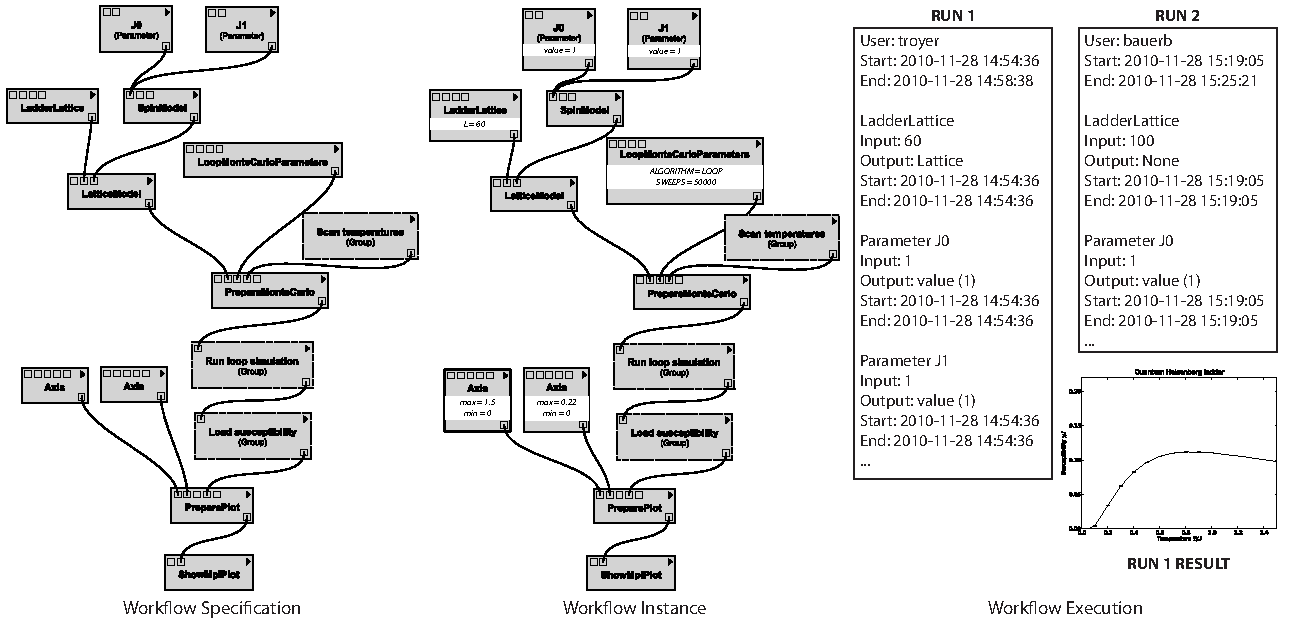
\includegraphics[width=\linewidth]{figures/alps_provenance_types.pdf}
\caption{The workflow specification (on the left) shows a workflow to calculate the uniform magnetic susceptibility of a quantum Heisenberg spin ladder and plot it as a function of temperature.
 The workflow
  instance (in the middle), in addition to the workflow specification,
  contains value assignments for parameters of the modules. This
  instance was used to derive the plot in the bottom right. The
  workflow runs (on the right) consist of information collected while
  the workflow instance was executed. }
\vspace{0cm}
\label{fig:workflow-spec-run}
\end{figure}

Formally, a \emph{workflow specification} is defined by a tuple
$(M,I,O,C,p:O \cup I \rightarrow M)$, where $M, I, O, C$ are,
respectively, sets of {\it modules}, {\it input ports}, {\it output
  ports}, {\it connections}, and $p$ is a function that assigns a
unique module to input and output ports.  If $x \in I \cup O$ and $m =
p(x)$ then we say that $x$ {\it is a port of module} $m$ and that $m$
is {\it the module of} $x$.  The set $C$ of connections is a subset of
$O \times I$.  In a {\it connection} $(o,i) \in C$, $o$ is called the
{\it source port} and $i$ is called the {\it target
  port}. Furthermore, the module of the source port cannot be the same
as the module of the target port.  An input port can be the target
port of at most one connection in $C$.  Additionally each port (input
or output) has an associated type and a {\it name} that is unique
across the ports of the same module.  A {\it module signature} is
defined as a set of pairs, where each pair contains a port name and
its type.  In addition, each module has a set of {\it parameters}.  Each parameter
has a unique {\it name} across the set of parameters of the same
module.

A \emph{workflow instance} consists of a specification combined with
bindings that provide values to parameters in the modules.  A {\it
  workflow run} is the execution of the following algorithm for a
workflow instance: each module checks whether all its input ports that
are target ports of a connection have a value; if false it waits; if
true, the module, according to its semantics, produces output values
on its output ports; values that are produced in an output port flow
to target ports of all the connections that have that output port as
its source port; this algorithm continues until there are no more
modules to execute.
%
These concepts are illustrated in Figure~\ref{fig:workflow-spec-run}.

\subsection{Data Provenance.}
In the context of scientific workflows, data provenance is a record of
the derivation of a set of results.  There are two distinct forms of
provenance~\cite{VDL:Challenge06}: prospective and retrospective.
\emph{Prospective provenance} captures the specification of a
computational task (\ie a workflow specification or instance)---it
corresponds to the \emph{steps that need to be followed} (or a recipe)
to generate a data product or class of data products.
\emph{Retrospective provenance} captures the \emph{steps that were
  executed} (\ie the workflow run) as well as information about the
execution environment used to derive a specific data product---a
detailed log of the execution of a computational task.

An important piece of information present in workflow provenance is
information about \emph{causality}: the dependency relationships
between data products and the processes that generate them.  Causality
can be inferred from both prospective and retrospective provenance.
Data provenance also includes \emph{user-defined information}, such as
documentation that cannot be automatically captured but records
important decisions and notes.  This data is often captured in the
form of annotations.

\paragraph{Provenance of Workflow Evolution.}
%
Although workflows have been traditionally used to automate repetitive
processes, for many exploratory scientific tasks such as data analysis
and visualization, change is the norm. As users formulate and test
hypotheses, they often need to refine and compare the results of
several workflows. VisTrails~\cite{vistrails} supports a novel
change-based provenance model that treats workflow instances as
first-class data
products~\cite{Freire:2006:IPAW,callahan@sciflow2006}.  As a scientist
makes modifications to a workflow, the system transparently records
those changes (\eg the addition of a module, the modification of a
parameter, \etc) akin to a database transaction log. Note that the
change-based model uniformly captures both changes to parameter values
and to workflow definitions. This sequence of changes is sufficient to
determine the provenance of data products, and it also captures
information about how the workflows evolve over time.  We refer to
this detailed provenance of the workflow evolution as a visual trail,
or a \emph{vistrail}.

\begin{figure}[t]
\centering
\begin{center}
  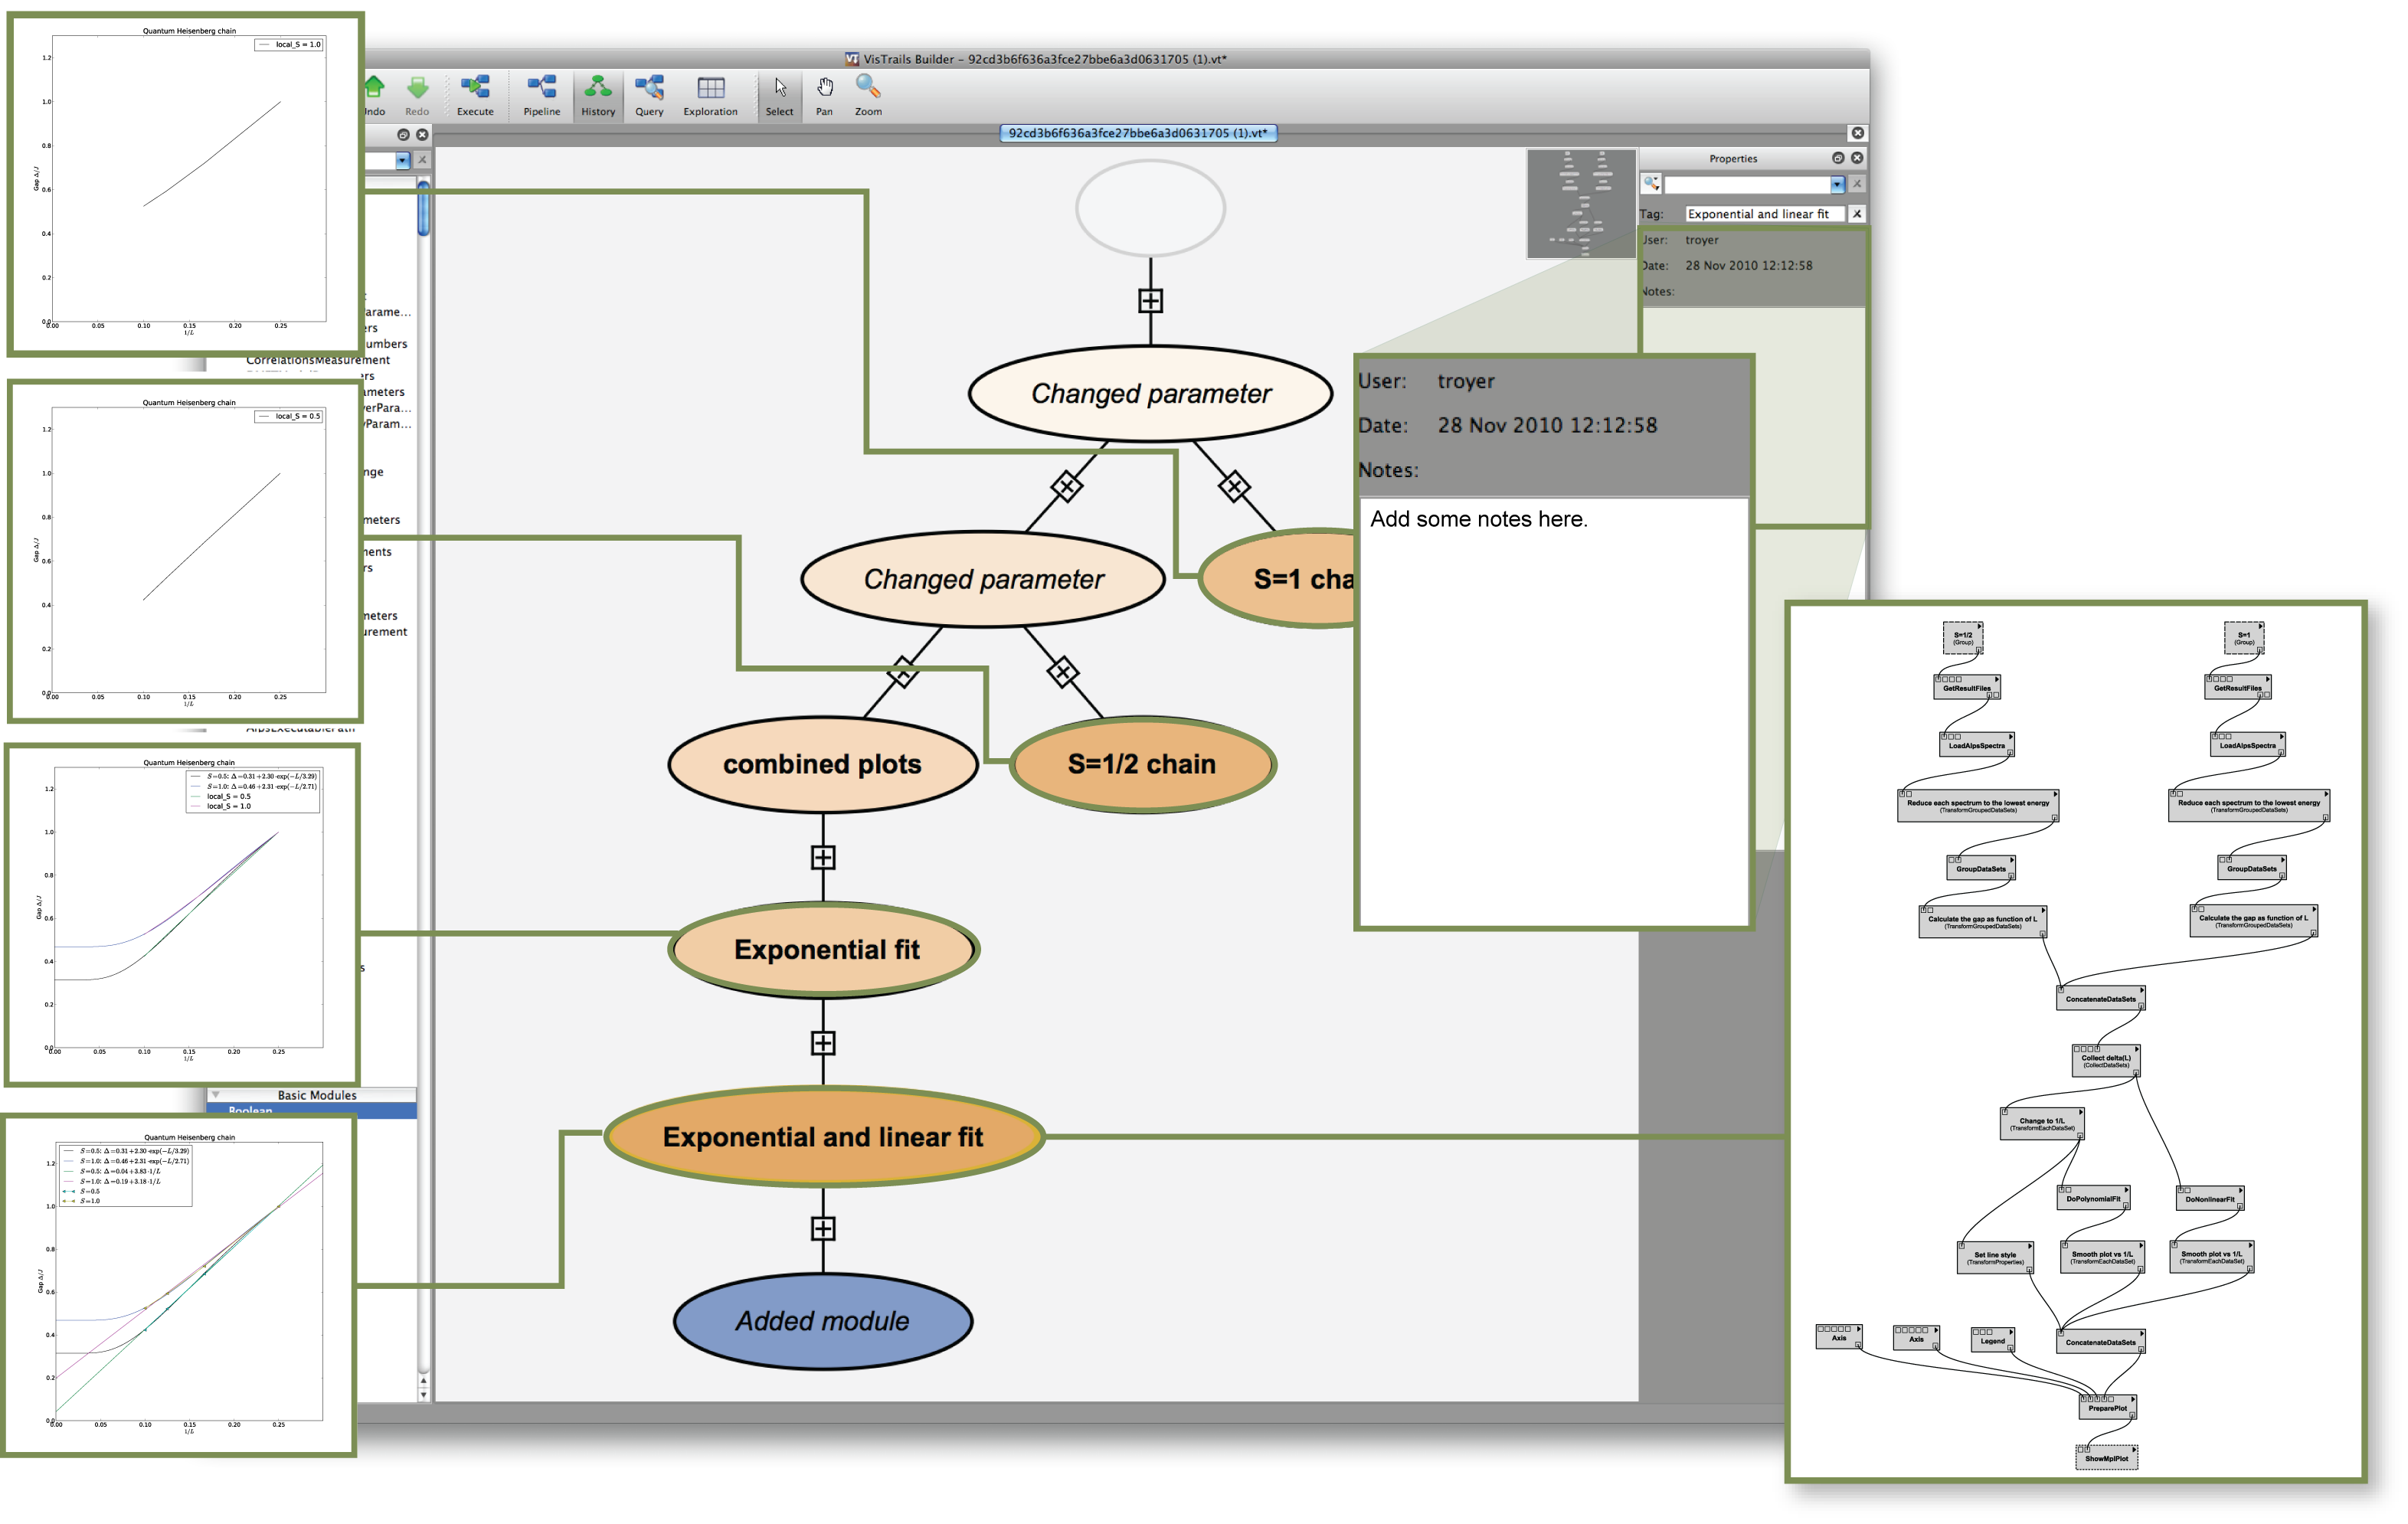
\includegraphics[width = 1.0\linewidth,clip=false]{figures/alps_tree.png}
  \caption{Workflow evolution provenance.  
    In this example we have calculated the system size dependence of the spin gap of spin-1 and spin 1/2 Heisenberg chains, first calculating the gap by exact diagonalization and then performing fits to $\Delta(L)=  c/L$ and  $\Delta(L)=  \Delta_0 + c \exp(-L/\xi)$. As expected from the Haldane conjecture the plots show that the first fit is best for the gapless spin-1/2 chain and the second fit is best for the gapped spin-1 chain.
    Complete provenance of the exploration process is
    displayed as a history tree with each node representing a workflow
    instance that generates a plot. Detailed meta-data is
    also stored including free-text notes made by the scientist, the
    date and time the workflow was created or modified, an optional
    descriptive tag, and the user that created it.} \label{fig:alps-tree}
  \vspace{-.3cm}
\end{center}
\end{figure}

As Figure~\ref{fig:alps-tree} illustrates, each node in a vistrail
corresponds to a workflow instance and contains value assignments for
the module parameters. A series of workflow runs may be associated
with a node as well as additional metadata, such as user annotations.
A tree-based view of a vistrail allows a scientist to return to a
previous version in an intuitive way, to undo bad changes, to compare
different workflows, and to be reminded of the actions that led to a
particular result.  Another important benefit of the change-based
provenance model is that it enables a series of operations that
simplify the exploration process, in particular, the ability to refine
workflows by analogy~\cite{analogies@tvcg2007}, as well as to visually
compare workflows and their results~\cite{Freire:2006:IPAW}.

It is important to note that the provenance of workflow execution and
workflow evolution help inform each other, leading to improved methods
for using the combined information. Knowing which workflow instances
have executed correctly can explain why workflows were updated, and
the number of times that an instance has been executed can help
highlight important versions of workflows.  Similarly, knowing how a
workflow evolved can help users debug errors that occur when running
modified versions.  Change-based provenance from workflow evolution
can also speed up runs of similar workflows via
caching~\cite{bavoil@vis2005}.

\begin{figure}
\begin{center}

\vistrail[host=alps.ethz.ch,
db=vistrails,
vtid=10,
version=169,
pdf,
getvtl,
showspreadsheetonly]{width=8cm}
\caption{A figure produced by an ALPS VisTrails workflow: the uniform susceptibility of the Heisenberg chain and ladder. Clicking the figure retrieves the workflow used to 
create it. Opening that workflow on a machine with VisTrails and ALPS installed lets the reader execute the full calculation.}
\label{fig:figure}
\end{center}
\end{figure}


\begin{figure}
\begin{center}
\vistrail[host=alps.ethz.ch,
db=vistrails,
vtid=10,
version=169,
pdf,
getvtl,
showworkflow,
showspreadsheetonly]{width=8cm}
\caption{The workflow that created Fig.~\ref{fig:figure}. The workflow image has been created by VisTrails for the specific workflow used to create the exact version shown in the figure. Clicking the figure retrieves the workflow.}
\label{fig:workflow}
\end{center}
\end{figure}



\begin{figure}
\begin{center}
\vistrail[host=alps.ethz.ch,
db=vistrails,
vtid=10,
version=172,
pdf,
getvtl,
showtree,
showspreadsheetonly]{width=8cm}
\caption{The version history tree of the workflow that created Fig.~\ref{fig:figure}. Each ellipsis corresponds to a version of the workflow, as shown in Fig.~\ref{fig:workflow}. Clicking the figure retrieves the vistrail including all workflow versions.}
\label{fig:history}
\end{center}
\end{figure}


\subsection{Caching and persistent storage}

%% We should discuss how VisTrails caches results, with the advantage
%% that only those parts of a workflow that have been changed have to be
%% re-executed - a big advantage over scripts. Also, we should mention
%% Dave's paper on strong links and persistent storage.

One important piece of infrastructure provided by VisTrails is the
management of data both used and produced by computational processes,
including intermediate results.  While parameters and workflow
structure may change from execution to execution, many of the
intermediate results can be reused without recomputation.  Note that
with traditional scripts, users must manually record and recall
intermediate results, meaning it is often necessary to repeat the
entire computation.  VisTrails supports efficient exploration of such
analyses by automatically caching intermediate results.  The results
in the cache are identified by the signature of the upstream
subworkflow (a hash computed from all of the computations that led to
the value).  If the signature exists in the cache, we need not compute
any of the upstream subworkflow but instead return the value in the
cache.  If anything in the subworkflow changes, the signature will
also change, and VisTrails will recompute the value.  VisTrails also
allows modules that are not deterministic to be flagged as
non-cacheable; note that all modules downstream of such modules must
also be recomputed each time.

In addition, VisTrails provides a persistence package to help users
manage their data and provide persistent caching.  This package
provides storage and versioning of input, intermediate, and output
data to ensure that workflows are able to access their data.  Data is
identified by unique ids rather than file paths, and users can name
and annotate the data in order to facilitate searching.  The data can
be linked to a local disk but is stored in a managed repository to
ensure that it is retained.  VisTrails will create new versions if
data changes, and provides persistent caching using the same signature
scheme as in-memory caching.  In contrast to the in-memory caching
mechanism, a persistent intermediate result can be recalled in later
sessions.  Using the metadata stored in persistent store and
provenance information, it is possible to connect data with the
workflows that either used or generated it and vice
versa~\cite{koop@ssdbm2010}.  In addition, users can not only trace
data lineage but also retrieve the exact input data---even if that
data was changed or removed on the filesystem.


\subsection{Sharing content and reproducible research}

One of the goals of the VisTrails system is to
facilitate the publication of scientific results. VisTrails and
CrowdLabs greatly simplify the process of packaging workflows and
results for publication. By supporting the publication on wikis, 
Web sites, or scientific documents (through LaTeX extensions such as in this paper), this framework allows users to create
documents whose digital artifacts (\eg figures) include a deep
caption: detailed provenance information which contains the
specification of the computational process (or workflow) and
associated parameters used to produce the
artifact. Figures~\ref{fig:figure} and \ref{fig:workflow} are examples
of this mechanism in action: both images were included by using
VisTrails directly and clicking on the images will download the
workflow with the parameters used to generate them. This workflow can then be used by the reader to reproduce the figures.

CrowdLabs is a social online workflow repository for the VisTrails
system. It combines workflow management tools with a scalable
infrastructure to allow scientists to collaboratively analyze and
visualize data. CrowdLabs is capable of hosting, executing, and
serving results from VisTrails workflows, including those that make
use of the ALPS VisTrails package. CrowdLabs also leverages provenance
information (\eg workflow/pipeline specifications, libraries,
packages, users, datasets and results) to provide a richer sharing
experience: users can search and query this information.

VisMashups \cite{Santos09}, another component developed on top of VisTrails, is a system for simplifying the creation,
maintenance and use of customized workflows. it is also
integrated into CrowdLabs and enables users to modify parameters and
re-execute workflows from within their web browsers. This provides an
entry point for non-experts to explore and interact with complicated
simulation workflows. We will develop ALPS tutorials also as VisMashups, enabling the interactive exploration of tutorial problems with the reader's web browser, without the need to install ALPS.


\subsection{The ALPS VisTrails package}

ALPS 2.0 provides a package of modules for VisTrails for the preparation of input files, the execution of simulations, and data analysis and plotting.

VisTrails workflows in ALPS 2.0 use descriptive nouns and verbs for the names of modules that execute
 Python scripts which, in turn execute ALPS
algorithms in Python or compiled code.  Fig.~\ref{fig:workflow} shows an example ALPS workflow
that takes input lattice parameters and model definitions (modules described by nouns, such as 
 ChainLattice and LatticeModel), executes the quantum
Monte Carlo looper code, and then renders the data (modules described by verbs such as  RunLoop and PreparePlot).

The creation of such workflows is explained in a set of tutorials and on the web page. Furthermore, all ALPS tutorials, discussed in the next section, are available  as VisTrails workflows, providing an extensive set of examples that can be used as templates for the user's simulations. 

This paper already makes use of ALPS 2.0 and VisTrails. Full provenance information for the results in Fig. \ref{fig:figure} is available from the URL linked to the figure. Clicking the figure will download the workflow that has been used to prepare the figure and its version history. After installing VisTrails and ALPS, the reader of the paper can redo the full simulation.


\section{Tutorials and Examples}

The ALPS web page \cite{alps} contains an extensive list of tutorials, explaining the use of the various application codes and evaluation tools.  Also, tutorials demonstrate how to use the ALPS libraries in the user's own code. We provide tutorials and instructions for using ALPS in three ways: 
\begin{enumerate}
\item from the command line (without data evaluation and plotting)
\item using Python scripts
\item and using the VisTrails workflow system. 
\end{enumerate}

The input files needed for the tutorials are available on the web page but are also included in the source and binary distributions.

\begin{figure}
\begin{tiny}
\begin{center}
\begin{verbatim}
cat  > parm << EOF
LATTICE="chain lattice"
MODEL="spin"
local_S=1/2
L=60
J=1
THERMALIZATION=5000
SWEEPS=50000
ALGORITHM="loop"
{T=0.05;}
{T=0.1;}
{T=0.2;}
{T=0.3;}
{T=0.4;}
{T=0.5;}
{T=0.6;}
{T=0.7;}
{T=0.75;}
{T=0.8;}
{T=0.9;}
{T=1.0;}
{T=1.25;}
{T=1.5;}
{T=1.75;}
{T=2.0;}
EOF

parameter2xml parm
loop --auto-evaluate --write-xml parm.in.xml
\end{verbatim}
\end{center}
\end{tiny}
\caption{A shell script to perform an ALPS simulation to calculate the uniform susceptibility of a Heisenberg spin chain. Evaluation options are limited to viewing the output files. Any further evaluation requires the use of Python, VisTrails, or a program written by the user.}
\label{fig:commandline}
\end{figure}


\begin{figure}
\begin{tiny}
\begin{center}
\begin{verbatim}
import pyalps
import matplotlib.pyplot as plt
import pyalps.plot

#prepare the input parameters
parms = []
for t in [0.05, 0.1, 0.2, 0.3, 0.4, 0.5, 0.6, 0.7, 0.8, 0.9, 1.0, 1.25, 1.5, 1.75, 2.0]:
    parms.append(
        { 
          'LATTICE'        : "chain lattice", 
          'MODEL'          : "spin",
          'local_S'        : 0.5,
          'T'              : t,
          'J'              : 1 ,
          'THERMALIZATION' : 5000,
          'SWEEPS'         : 50000,
          'L'              : 60,
          'ALGORITHM'      : "loop"
        }
    )

#write the input file and run the simulation
input_file = pyalps.writeInputFiles('parm2c',parms)
pyalps.runApplication('loop',input_file)

#load the susceptibility and collect it as function of temperature T
data = pyalps.loadMeasurements(pyalps.getResultFiles(prefix='parm2c'),'Susceptibility')
susceptibility = pyalps.collectXY(data,x='T',y='Susceptibility')

#make plot
plt.figure()
pyalps.plot.plot(susceptibility)
plt.xlabel('Temperature $T/J$')
plt.ylabel('Susceptibility $\chi J$')
plt.title('Quantum Heisenberg chain')
plt.show()
\end{verbatim}
\end{center}
\end{tiny}
\caption{A Python script to perform an ALPS simulation to calculate the uniform susceptibility of a Heisenberg spin chain, load and evaluate the data, and make a plot. }
\label{fig:python}
\end{figure}

An example for running an ALPS application from the command line is shown in Fig.~\ref{fig:commandline}. This example calculates the uniform susceptibility of a quantum Heisenberg spin chain. The same example, containing additional code to evaluate and plot the results  using Python is shown in Fig.~\ref{fig:python}. The workflow using VisTrails is shown in Fig.~\ref{fig:workflow}, and its version history in Fig.~\ref{fig:history}. Following the links in the PDF version of the latter figures retrieves the corresponding vistrail files.

\section{License}
The ALPS libraries are licensed under the ALPS library license \cite{librarylicense} and the applications under the ALPS application license  \cite{applicationlicense}. These licenses are modeled after the GNU General Public License (GPL), but contain an additional requirement to cite this paper as well as relevant papers for each of the application codes. These papers need to be cited and the use of ALPS acknowledged in any scientific project that makes use of ALPS. This includes the case when ALPS has only been used to test a scientist's application code.

The detailed license text is included in the files {\tt LICENSE.txt} \cite{librarylicense} and {\tt LICENSE-applications.txt}  \cite{applicationlicense}. Any use of ALPS requires citing this paper.  These files can be found at the top level of the source distribution and in the directory {\tt share/alps} of the binary distributions. The papers that need to be cited for the use of a specific application are printed to the standard output when that application is run. The list of papers is also included in the file {\tt CITATIONS.txt}. Since some of those references are to preprints we recommend that the ALPS web page \cite{alps} is checked for updates.

\section{Future development plans}

The ALPS project is a work in progress and development will continue after this release 2.0. Immediate plans for release 2.1 within about a year include the development of  more evaluation tools for Monte Carlo simulations and more 2D and 3D plotting functionality.

ALPS 2.1 will also provide support for more programming languages. In addition to the Python support in the current version we plan to add a Fortran library to write the ALPS HDF5 files from Fortran. This will enable the use of the ALPS evaluation tools not only with C++ or Python codes, but also with results of Fortran codes.

A key part of ALPS 2.1 will be a more flexible and optimized scheduler. It will allow  the simple integration of the ALPS codes into other programs and Python scripts. It is also designed to scale to tens of thousands of CPUs, compared to the current scheduler that scales only to a few thousand CPUs. 

Besides improved versions of some of the simulation codes, there will be a new worm algorithm program for optical lattice simulations with millions of lattice sites, and an extension of the DMFT codes to clusters.

ALPS is an open initiative and we welcome contributions from the community.


\section{Acknowledgements}

We thank A.F. Albuquerque, F. Alet, P. Corboz, P.Dayal, A. Honecker, A. L\"auchli, M. K\"orner,  A. Kozhevnikov, S. Manmana, M. Matsumoto, I.P. McCulloch, F. Michel and R.M. Noack, for their contributions to previous versions of ALPS and  for useful discussions. 

We thank all users of the previous versions of ALPS and beta testers of ALPS 2.0, especially J. Alfonsi, S. Aicardi, A. Akande, P. Anders, A. Anfossi, Z. Asadzadeh, R.~Bhat, J.H. Brewer, S. Bulut, E. Burovski, G. Carleo, G. Chen, M.D. Costa, M.~Dolfi, J. Figgins, S.~Gazit, U.~Gerber, R. Ghulghazaryan, C. Gils, S. Greschner, C.~Hamer, J. Hammond, K. Hassan, N. Heine, F.-J. Jiang, R. Jordens, H.G. Katzgraber, B.~Keiyh, J. Kim, J. Kolasinski, B.~Koopman, F. K\"ormann E.~Kozik, M.F. Krenn, F.~Kruger, M. Laurent, J. Lopes, M. Maik, M. Maksymenko, N. Moran, A. Nunnenkamp, J.D. Peel, S.~Pilati, K. Prsa, N.~Rahman, M. Rofiq, H. R\o nnow, J. Ruostekoski, J.~Schnack, N. Schuch, A. Sen, K. Shtengel, J. Single, M. Skoulatos, C. Sliwa, M.~Spenke, M.~Stoudenmire, V. Tangoulis, A.~Taroni, B. Thielemann, M. Tovar, H. Tran, V.~Varma, S. Ward, T. Wasiutynski, J. Wen, J. Wilms, H. Wunderlich, F. Xiao, X.Q. Yu, J.~Zakrzewski, Z.-X. Zhou, and R. Ziemkiewicz. We thank P. Zoller for the suggestion to provide binary installers. 

The development of ALPS has profited from support of the Pauli Center at ETH Z\"urich, the Swiss HP$^2$C initiative, the Kavli Institute for Theoretical Physics in Santa Barbara supported by NSF grant  PHY-0551164 and DMR-0705847, the Aspen Center for Physics, the Swiss National Science Foundation, the Jeffress Memorial Trust, Grant No.~J-992, the National Science Foundation under Grant No.~PHY-0903457, the Deutsche Forschungsgemeinschaft through the collaborative research center SFB 602, Japan Society for the Promotion of Science through KAKENHI No.\,20540364, Next-Generation Supercomputer Project from MEXT Japan, and a grant from the Army Research Office with funding from the DARPA OLE program.


\section*{References}

\bibliographystyle{iopart-num}
\bibliography{refs}
\end{document}
